% Template for ICIP-2015 paper; to be used with:
%          spconf.sty  - ICASSP/ICIP LaTeX style file, and
%          IEEEbib.bst - IEEE bibliography style file. cambio para probar adsfasfasfasfsf
% --------------------------------------------------------------------------
\documentclass[spanish]{article}
\usepackage{spconf,amsmath,graphicx}
\usepackage{mathptmx}
\usepackage{mathtools}
\usepackage{amsmath}
\usepackage{mathrsfs}
\usepackage{amssymb}
\usepackage{amsfonts}
\usepackage[utf8]{inputenc}
\usepackage{babel}
\selectlanguage{spanish}
% Example definitions.
% --------------------
\def\x{{\mathbf x}}
\def\L{{\cal L}}

% Title.
% ------
\title{OPTIMIZACIÓN MULTIOBJETIVO BASADA EN LA SINTONIZACIÓN DE LOS PARÁMETROS DE CLAHE PARA OBTENER DISTINTOS NIVELES DE CONTRASTE EN RADIOGRAFIA DEL TORAX}
%\title{OPTIMIZACIÓN MULTIOBJETIVO PARA LA MEJORA DEL CONTRASTE BASADA EN CLAHE.}
%
% Single address.
% ---------------
\name{Luis G. Moré, Marcos A. Brizuela, José Luis Vázquez Noguera, Diego Pinto-Roa, Horacio Legal Ayala}
\address{Facultad Politécnica - Universidad Nacional de Asunción}
%
% For example:
% ------------
%\address{School\\
%	Department\\
%	Address}
%
% Two addresses (uncomment and modify for two-address case).
% ----------------------------------------------------------
%\twoauthors
%  {A. Author-one, B. Author-two\sthanks{Thanks to XYZ agency for funding.}}
%	{School A-B\\
%	Department A-B\\
%	Address A-B}
%  {C. Author-three, D. Author-four\sthanks{The fourth author performed the work
%	while at ...}}
%	{School C-D\\
%	Department C-D\\
%	Address C-D}
%
\begin{document}
%\ninept
%
\maketitle
%
\begin{abstract}
La mejora del contraste en imágenes médicas presenta desafíos importantes, debido a que se necesita realzar los detalles y también preservarlos, de forma a que la mejora sea de ayuda para análisis posteriores. Se propone un enfoque de mejora multiobjetivo basada en CLAHE, utilizando SMPSO como metaheurística, además de la Entropía y el SSIM como objetivos, de manera a maximizar el contraste y minimizar la distorsión de los resultados. Se obtienen distintos niveles de contraste en imágenes de radiografía del tórax, y así se resaltan distintos detalles de éstas. Los resultados obtenidos se analizan con ayuda de un especialista de manera a determinar la utilidad del enfoque, además se verifica que los objetivos son contradictorios.
\end{abstract}
%
\begin{keywords}
SMPSO,CLAHE,Entropía,SSIM, Mejora del Contraste, Optimización.
\end{keywords}
%
\section{Introducción}
\label{sec:intro}

Los aparatos médicos se pueden conectar a computadoras y digitalizar las imágenes que construyen \cite{garcia_fenoll,russ2010}; sin embargo, la captura de la imagen a través de éstos dispositivos no está exenta de problemas: la captura puede sufrir de adición de ruido, mucha oscuridad, bajo contraste, entre otros. Por tanto, es necesario realizar un procesamiento previo de manera a que las imágenes puedan ser analizadas posteriormente; ésto es particularmente importante para las imágenes médicas, debido a la cantidad de detalles finos e importantes que poseen.

Contrast Limited Adaptive Histogram Equalization (CLAHE) es un algoritmo de mejora de contraste local basado en la división de la imagen en bloques y la ecualización del histograma de cada bloque en forma independiente, el cual fué propuesto en \cite{Zuiderveld:1994:CLA:180895.180940}. CLAHE ha demostrado obtener buenos resultados principalmente en imágenes con bajo contraste \cite{balvant2011} e imágenes médicas \cite{saikat2011,shelda2013}, debido a que en este último grupo se priorizan los detalles de la imagen. Una característica importante de CLAHE es que posee dos parámetros de entrada que controlan la mejora del contraste que se obtiene como resultado. De manera a obtener una solución satisfactoria se deben escoger valores apropiados de éstos parámetros. Debido a que el rango de parámetros a elegir es sumamente amplio, se necesita de una metaheurística que permita encontrar valores de entrada de CLAHE que arrojen los resultados más satisfactorios de manera efectiva.
\section{estado del arte}

\section{contrast limited adaptive histogram equalization}
\label{sec:clahe}

El comportamiento natural en el ojo humano es el de evaluar la información que se muestra en una imagen, basándose en los componentes locales presentes. Por tanto es relevante realizar la mejora del contraste en base a los componentes locales de la imagen. En el Adaptive Histogram Equalization (AHE), éste método se implementa utilizando secciones rectangulares de la imagen denominadas {\it Regiones Contextuales}, cuyas dimensiones podemos definir como $(\mathcal{R}_x, \mathcal{R}_y)$. Luego se realiza la Ecualización del Histograma utilizando los pixeles que se encuentran dentro de la región contextual. Además se utiliza un esquema de interpolación bilineal, de manera a corregir inconsistencias en las fronteras entre regiones. Una de las características de AHE es que es capaz de aumentar la información contenida dentro de la imagen, a través de la mejora del contraste\cite{zimmerman1988evaluation}.

AHE es un algoritmo que presenta problemas de amplificación del ruido, el cual es más visible en regiones en donde se encuentras niveles de gris relativamente homogéneos. Ésta limitación puede solucionarse si se utiliza un esquema de limitación de contraste dentro de las regiones contextuales. Por tanto, en CLAHE se implementa una limitación en el contraste a través de la limitación de la cantidad de pixeles que pueden alcanzar cierto nivel de gris dentro del histograma local, por lo que se corrige el problema de los picos en el histograma asociados a las regiones con niveles de gris homogéneos. Los pixeles que superan cierto umbral se recortan para eliminar picos, y se redistribuyen de forma equitativa a través del histograma ecualizado de la región contextual. Entonces podemos definir el {\it Clip Limit} $\mathcal{C}$ como un factor que está fuertemente relacionado con los contenidos del histograma. Si definimos un coeficiente $\mathcal{C}$ relativamente bajo, entonces los histogramas de las regiones contextuales no muestran picos, por lo que se obtiene una mejora del contraste relativamente suave. Si definimos un $\mathcal{C}$ alto, obtenemos un comportamiento de $CLAHE$ que resulta ser equivalente al algoritmo $AHE$.

A continuación se muestran las métricas de evaluación utilizadas como objetivo para evaluar la calidad de las soluciones encontradas utilizando la metodología propuesta.

\section{métricas de evaluación}
\label{sec:metricas}

\subsection{entropía}
\label{ssec:entropia}

La {\it Entropía de la Información} es un coeficiente que arroja una medida de la aleatoriedad que se presenta en la señal que acarrea una imagen \cite{tsai2008information}. Si medimos la entropía que arrojan 2 imágenes cualitativamente similares, podemos evaluar si existe una mejora en la cantidad de información que provee la imagen con el contraste mejorado. En las imágenes en escala de gris, la {\it Entropía} se define como un coeficiente que muestrá cuántos niveles de gris de los que se encuentran disponibles para representar la imagen se usan de manera efectiva \cite{kwok2006intensity}.

De manera previa a la formulación de la {\it Entropía de la Información} en el contexto de las imágenes en escala de gris, necesitamos definir el histograma de una imagen, como se muestra en \eqref{eq:histograma}:

\begin{equation}\label{eq:histograma}
    \mathcal{H}=\{h_i \in [0...N]\mid i=0,1,...,L-1\}
\end{equation}

Donde $h_i$ es el conteo de courrencias del $i-esimo$ nivel de gris que compone la imagen; $N$ es el número total de pixeles de la imagen (nótese que $N=\sum_{i=0}^{L-1}h_i$); $L$ es el nivel de gris más alto utilizado para representar los niveles de gris en la imagen. En una escala de 8 bits, el nivel máximo representable es $2^8=256$ niveles posibles. Así, la distribución normal de niveles de gris del histograma se define como: 

\begin{equation}\label{eq:distribucionormal}
\mathcal{P}_i=\frac{h_i}{N}
\end{equation}

finalmente, podemos formular la entropía de la imagen dada como \eqref{eq:entropia}:

\begin{equation}\label{eq:entropia}
\mathscr{H}=-\sum_{i=0}^{L-1}\mathcal{P}_i log_2(\mathcal{P}_i) [bits]
\end{equation}

Es importante realizar la medición de la Entropía de la imagen, porque está directamente relacionada con la homogeneidad en el brillo medio \cite{108593}. 

Ésta métrica por sí sola no es suficiente para evaluar la calidad de las soluciones encontradas, debido a que no mide la distorsión producida por la mejora en el contraste de la imagen. Por tanto, es necesario adoptar otra métrica, la cual se muestra en la sección siguiente. 

\subsection{índice de similitud estructural}
\label{ssec:ssim}

El Índice de Similitud Estructural (SSIM) es un coeficiente con el cual se puede realizar la evaluación de cambios introducidos en la información estructural, por lo que da una medida adecuada de la distorsión producida en la imagen a consecuencia de la Mejora del Contraste. SSIM se basa en la noción de que existe una dependencia fuerte entre pixeles que conforman una vecindad \cite{kwok2013locally}. Los métodos tradicionales de evaluación de la distorsión como Peak Signal to Noise Ratio (PSNR), el Error Cuadrático Medio (MSE) y sus derivados, son inconsistentes con la percepción de la visión humana \cite{}

\section{Formulación}
\label{sec:formulacion}

Dadas la imagen de entrada $I$ y el algoritmo $CLAHE$, se desea calcular el conjunto de soluciones $\mathscr{X}$ que maximice de manera simultánea los objetivos $\mathscr{H}$ y $\mathcal{C}$, como se muestra abajo:

\begin{equation}\label{eq:fitness}
    f(\overrightarrow{x}) = \{ f_1(\overrightarrow{x}), f_2(\overrightarrow{x}) \}
\end{equation}

donde:
\begin{itemize}
\item $\overrightarrow{x}=(\mathcal{R}_x, \mathcal{R}_y, \mathcal{C})$, donde $\mathcal{R}_x$ y $\mathcal{R}_y$ conforman la región contextual y $\mathscr{C}$ es el Clip Limit.
\item $f_{1}(\overrightarrow{x})=\frac{\mathscr{H}(T)}{log_{2}L}$ es la Entropía normalizada de la imagen $T$, siendo $T$ la imagen mejorada por $CLAHE$ con los parámetros dados por $\overrightarrow{x}$, y $L$ la cantidad de grises disponibles.
\item $f_{2}(\overrightarrow{x})=SSIM(I,T)$ es el Índice de Similitud Estructural.
\end{itemize}

sujeto a:

\begin{itemize}
\item $\mathcal{R}_x \in [2,..,M]$ en los números $\mathbb{N}$.
\item $\mathcal{R}_y \in [2,..,N]$ en los números $\mathbb{N}$.
\item $\mathscr{C} \in (0,1]$ en los números $\mathbb{R}$.
\end{itemize}

Ésto significa que los valores de $\mathcal{R}$ solamente pueden tomar valores enteros positivos entre $(2,2)$ y $(M,N)$ y que $\mathscr{C}$ puede tomar un valor mayor a cero y menor o igual a 1.

\section{optimización de enjambre de partículas multiobjetivo}
\label{sec:pagestyle}

\section{propuesta}
\label{sec:typestyle}


\section{resultados y discusión}
\label{sec:majhead}


\subsection{Subheadings}
\label{ssec:subhead}

 

\section{conclusiones}
\label{sec:print}


% Below is an example of how to insert images. Delete the ``\vspace'' line,
% uncomment the preceding line ``\centerline...'' and replace ``imageX.ps''
% with a suitable PostScript file name.
% -------------------------------------------------------------------------
%\begin{figure}[t]

%\begin{minipage}[b]{1.0\linewidth}
%  \centering
%  \centerline{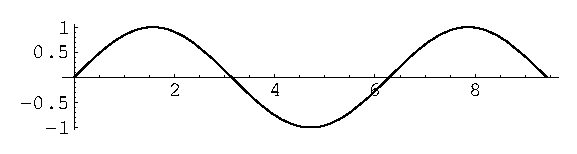
\includegraphics[width=8.5cm]{Figures/image1}}
%  \vspace{2.0cm}
%  \centerline{(a) Result 1}\medskip
%\end{minipage}
%
%\begin{minipage}[b]{.48\linewidth}
%  \centering
%  \centerline{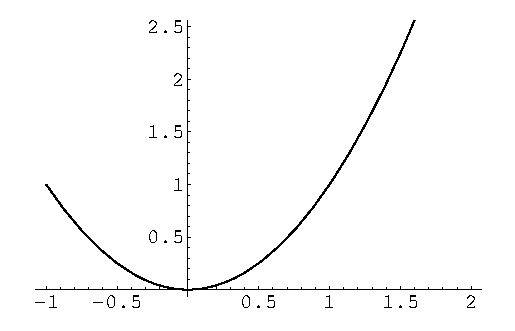
\includegraphics[width=4.0cm]{Figures/image3}}
%  \vspace{1.5cm}
%  \centerline{(b) Results 3}\medskip
%\end{minipage}
%\hfill
%\begin{minipage}[b]{0.48\linewidth}
%  \centering
%  \centerline{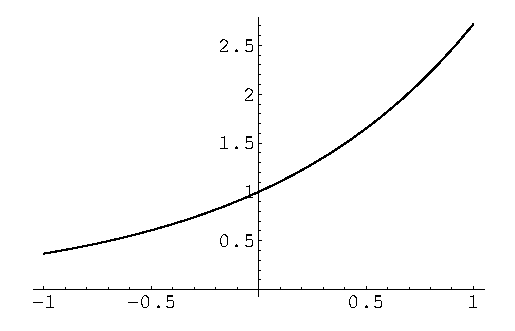
\includegraphics[width=4.0cm]{Figures/image4}}
%  \vspace{1.5cm}
%  \centerline{(c) Result 4}\medskip
%\end{minipage}
%
%\caption{Example of placing a figure with experimental results.}
%\label{fig:res}
%
%\end{figure}


% To start a new column (but not a new page) and help balance the last-page
% column length use \vfill\pagebreak.
% -------------------------------------------------------------------------
%\vfill
%\pagebreak

\section{COPYRIGHT FORMS}
\label{sec:copyright}

You must include your fully completed, signed IEEE copyright release form when
form when you submit your paper. We {\bf must} have this form before your paper
can be published in the proceedings.

\section{REFERENCES}
\label{sec:ref}

List and number all bibliographical references at the end of the
paper. The references can be numbered in alphabetic order or in
order of appearance in the document. When referring to them in
the text, type the corresponding reference number in square
brackets as shown at the end of this sentence \cite{C2}. An
additional final page (the fifth page, in most cases) is
allowed, but must contain only references to the prior
literature.

% References should be produced using the bibtex program from suitable
% BiBTeX files (here: refs). The IEEEbib.bst bibliography
% style file from IEEE produces unsorted bibliography list.
% -------------------------------------------------------------------------
\bibliographystyle{IEEEbib}
\bibliography{refs}

\end{document}
